\taskpic{ Две заряженных частицы: одна массой $M$ и зарядом $+Q$, другая
  массой $m$ и зарядом $-q$ помещены в постоянное однородное
  электрическое поле $E$. Частицы отпускают, и они остаются на
  постоянном расстоянии $L$ друг от друга. Чему равно это расстояние?
}
{
  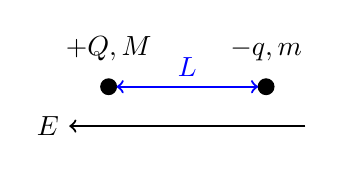
\begin{tikzpicture}
    \draw[fill=black] (0,0) circle (0.1) node[above=0.2cm] {$+Q,M$};
    \draw[fill=black] (2,0) circle (0.1) node[above=0.2cm] {$-q,m$};
    \draw[thick,blue,<->] (0.1,0) -- (1.9,0) node[above,midway] {$L$};
    \draw[thick,->] (2.5,-0.5) -- (-0.5,-0.5) node[left] {$E$};
  \end{tikzpicture}
}
% Physics Challengs, TPT, January 2002
